\documentclass{article}
\usepackage{graphicx}
\usepackage{bm}
\usepackage{amsmath}
\usepackage{amssymb}
\usepackage[toc,page]{appendix}
\usepackage{listings}
\usepackage{color}
\usepackage{listings}
\usepackage{fullpage}

\numberwithin{equation}{subsection}

\definecolor{mygreen}{rgb}{0,0.6,0}
\definecolor{mygray}{rgb}{0.5,0.5,0.5}
\definecolor{mymauve}{rgb}{0.58,0,0.82}

\lstset{ %
  backgroundcolor=\color{white},   % choose the background color; you must add \usepackage{color} or \usepackage{xcolor}
  basicstyle=\footnotesize,        % the size of the fonts that are used for the code
  breakatwhitespace=false,         % sets if automatic breaks should only happen at whitespace
  breaklines=true,                 % sets automatic line breaking
  captionpos=b,                    % sets the caption-position to bottom
  commentstyle=\color{mygreen},    % comment style
  deletekeywords={...},            % if you want to delete keywords from the given language
  escapeinside={\%*}{*)},          % if you want to add LaTeX within your code
  extendedchars=true,              % lets you use non-ASCII characters; for 8-bits encodings only, does not work with UTF-8
  frame=single,	                   % adds a frame around the code
  keepspaces=true,                 % keeps spaces in text, useful for keeping indentation of code (possibly needs columns=flexible)
  keywordstyle=\color{blue},       % keyword style
  language=Octave,                 % the language of the code
  otherkeywords={*,...},            % if you want to add more keywords to the set
  numbers=left,                    % where to put the line-numbers; possible values are (none, left, right)
  numbersep=5pt,                   % how far the line-numbers are from the code
  numberstyle=\tiny\color{mygray}, % the style that is used for the line-numbers
  rulecolor=\color{black},         % if not set, the frame-color may be changed on line-breaks within not-black text (e.g. comments (green here))
  showspaces=false,                % show spaces everywhere adding particular underscores; it overrides 'showstringspaces'
  showstringspaces=false,          % underline spaces within strings only
  showtabs=false,                  % show tabs within strings adding particular underscores
  stepnumber=2,                    % the step between two line-numbers. If it's 1, each line will be numbered
  stringstyle=\color{mymauve},     % string literal style
  tabsize=2,	                   % sets default tabsize to 2 spaces
  title=\lstname                   % show the filename of files included with \lstinputlisting; also try caption instead of title
}

\begin{document}

\title{Discrete Ordinates}
\author{Edward Norris}

\maketitle

\begin{abstract}
The abstract text goes here.
\end{abstract}

\tableofcontents

\section{CODE}
Consider that we have the following variables, $\Psi$ which is a function of $x$, $y$, $z$, $E$, and $\hat{\Omega}$. Further, we have the in-flux variables $\Psi_{x-in}$, $\Psi_{y-in}$, and $\Psi_{z-in]}$. 

Given:
\begin{itemize}
\item A list of all energies, $\mathcal{E}$
\item A list of all directions in the quadrature, $Q$
\item A mapping from $r$ to zone number, $\mathcal{Z}(r)$
\item Lists of direction cosines, $\mu$, $\xi$, and $\eta$
\item A map of $r$ to voxel volume, $V(r)$
\item A list of all $x$, $y$, and $z$ voxel centers, $X$, $Y$, and $Z$
\item A list of weights for the quadrature, $\omega$
\item A list of scatter cross sections in zone $\mathcal{Z}(r)$ from energy $E'$ to $E$, $\Sigma_s(\mathcal{Z}(r), E', E)$
\item A list of total cross sections in zone $\mathcal{Z}(r)$ at energy $E$, $\Sigma_T(\mathcal{Z}(r), E)$
\item The surface area of all voxels, $A_{xy}(r)$, $A_{yz}(r)$, $A_{xz}(r)$
\end{itemize}

\pagebreak
\begin{lstlisting}[escapeinside={(*}{*)}]
function sweep()

  (*$\phi(r, E) = \vec{0}$*)    # Scalar flux
  (*$\Psi(r, \Omega, E) = \vec{0}$*)  # Angular flux
  
  for (*$E \in \mathcal{E}$*) in descending order
    while not converged
      for (*$\Omega \in Q$*) in any order
        if (*$\mu(\Omega) > 0$*) and (*$\xi(\Omega) > 0$*) and (*$\eta(\Omega) > 0$*)
          octant1()
        else if (*$\mu(\Omega) > 0$*) and (*$\xi(\Omega) > 0$*) and (*$\eta(\Omega) < 0$*)
          octant2()
        ...
        else
          octant8()
\end{lstlisting}

\pagebreak
\begin{lstlisting}[escapeinside={(*}{*)}]
function octant1()

  for (*$x \in X$*) in ascending order
    for (*$y \in Y$*) in ascending order
      for (*$z \in Z$*) in ascending order
            
        (*$S$*) = totalScatter((*$x, y, z, \Omega, E$*))            
            
        # Get the in-flux from the previous out-flux
        (*$\Psi_{x-in}(x, y, z, E, \Omega) \leftarrow \Psi_{x-out}(x-\Delta x, y, z, E, \Omega)$*)
        (*$\Psi_{y-in}(x, y, z, E, \Omega) \leftarrow \Psi_{x-out}(x, y-\Delta y, z, E, \Omega)$*)
        (*$\Psi_{z-in}(x, y, z, E, \Omega) \leftarrow \Psi_{x-out}(x, y, z-\Delta z, E, \Omega)$*)
              
        # Calculate the angular flux
        (*$n \leftarrow S + 2\mu(\Omega)A_{yz}(y,z)\Psi_{x-in}(x,y,z,E,\Omega) + $*)
               (*$2\xi(\Omega)A_{xz}(x,z)\Psi_{y-in}(x,y,z,E,\Omega) + $*)
               (*$2\eta(\Omega)A_{xy}(x,y)\Psi_{z-in}(x,y,z,E,\Omega)$*)
        (*$d \leftarrow 2\mu(\Omega)A_{yz}(y,z) + 2\xi(\Omega)A_{xz}(x,z) + 2\eta(\Omega)A_{xy}(x,y) + \Sigma_T(\mathcal{Z}(r), E)$*)
        (*$\Psi(x, y, z, E, \Omega) \leftarrow n/d $*)
              
        # Calculate the out-flux
        (*$\Psi_{x-out}(x, y, z, E, \Omega) \leftarrow 2 \Psi(x, y, z, E, \Omega) - \Psi_{x-in}(x, y, z, E, \Omega)$*)
        (*$\Psi_{y-out}(x, y, z, E, \Omega) \leftarrow 2 \Psi(x, y, z, E, \Omega) - \Psi_{y-in}(x, y, z, E, \Omega)$*)
        (*$\Psi_{z-out}(x, y, z, E, \Omega) \leftarrow 2 \Psi(x, y, z, E, \Omega) - \Psi_{z-in}(x, y, z, E, \Omega)$*)
            
        # Increment the scalar flux
        (*$\phi(x, y, z, E) \leftarrow \phi(x, y, z, E) + \omega(\Omega) \Psi(x, y, z, E, \Omega)$*)
\end{lstlisting}

\pagebreak
\begin{lstlisting}[escapeinside={(*}{*)}]
function totalScatter((*$r, \Omega, E$*))

  # Assume a point source at (*\color{mygreen} $r_0$*) with energy (*\color{mygreen} $E_0$*) and strength (*\color{mygreen} $S_0$*) particles / sec
  (*$S_x \leftarrow 0$*)
  if (*$r = r_0$*) and (*$E = E_0$*)
    (*$S_x \leftarrow (1/4\pi) \times S_0$*)

  (*$S_D \leftarrow 0$*)
  for (*$E' \in \mathcal{E} | E' \geq E$*)
    (*$S_D = S_D + (1/4\pi) \times \phi(r, \Omega, E') \times \Sigma_s(\mathcal{Z}(r), E', E) \times V(r)$*)
    
  (*$S_T = S_x + S_D$*)
  return (*$S_T$*)
\end{lstlisting}

\section{Introduction}
This document will teach you everything you need to know about the Boltzmann Equation from its derivation to the details of its implementation in computer code.

\section{Mathematical Development}

\subsection{The Boltzmann Equation}

The time dependent gamma transport equation can be written as

\begin{equation} \label{eq_boltz_t_dep}
\begin{split}
	&\left[ \frac{1}{v(E)} \frac{\partial}{\partial t} + \hat{\Omega} \cdot \nabla + \Sigma_t(\boldsymbol{r}, E, t) \right]
	\psi(\boldsymbol{r}, E, \hat{\Omega}, t) = \\
	&\int_{4 \pi} \int_0^\infty \Sigma_s(\boldsymbol{r}, E' \rightarrow E, \hat{\Omega}' \rightarrow \hat{\Omega}, t) \psi(\boldsymbol{r}, E', \hat{\Omega}', t) dE' d\hat{\Omega}' + S(\boldsymbol{r}, E, \hat{\Omega}, t)
\end{split}
\end{equation}

However, we are typically not concerned with the transient case in medical diagnostic imaging. We are more interested in the steady state case. The time independent form of Eq. \ref{eq_boltz_t_dep} is written as

\begin{equation} \label{eq_boltz}
\begin{split}
	&\left[ \hat{\Omega} \cdot \nabla + \Sigma_t(\boldsymbol{r}, E) \right]
	\psi(\boldsymbol{r}, E, \hat{\Omega}) = \\
	&\int_{4 \pi} \int_0^\infty \Sigma_s(\boldsymbol{r}, E' \rightarrow E, \hat{\Omega}' \rightarrow \hat{\Omega}) \psi(\boldsymbol{r}, E', \hat{\Omega}') dE' d\hat{\Omega}' + S(\boldsymbol{r}, E, \hat{\Omega})
\end{split}
\end{equation}

\subsection{Harmonic Approximation}
Equation \ref{eq_boltz} has a number of terms that cannot be solved directly. Instead, some numerical approximation must be used. The macroscopic scattering cross section, $\Sigma_s$ is typically expanded with a Legendre polynomial (for more information of Legendre polynomials, refer to Section \ref{sec_legendre}). The expansion is as follows:

\begin{equation} \label{eq_sigma_expansion}
\Sigma_s(\boldsymbol{r}, E' \rightarrow E, \hat{\Omega}' \rightarrow \hat{\Omega}) \approx \sum_{l=0}^L \frac{2l+1}{4 \pi} \Sigma_{s,l}(\boldsymbol{r}, E' \rightarrow E) P_l(\hat{\Omega}' \rightarrow \hat{\Omega})
\end{equation}

where $\Sigma_{s,l}$ is the expansion coefficients termed the "scattering moments." The Legendre polynomials $P_l(\hat{\Omega}' \rightarrow \hat{\Omega}$ are defined as

\begin{equation} \label{eq_harmonic}
P_l(\hat{\Omega}' \rightarrow \hat{\Omega}) = \frac{1}{2l+1}\sum_{m=-l}^l Y_{l,m}^*(\hat{\Omega}')Y_{l,m}(\hat{\Omega})
\end{equation}

The angular fluence ($\phi$) is also expanded as

\begin{equation}
\phi(\boldsymbol{r}, E', \hat{\Omega}') \approx \sum_{l=0}^L \sum_{m=-l}^l
\phi_{lm}(\boldsymbol{r}, E')Y_{lm}(\hat{\Omega}')
\end{equation}

\noindent
A source term suitable for numeric integration is then

\begin{equation}\label{eq_harmonic_simp1}
\begin{split}
\int_0^\infty dE' \int_{4 \pi} d\hat{\Omega}' \Sigma_s(\boldsymbol{r}, E' \rightarrow E, \hat{\Omega}' \rightarrow \hat{\Omega}) \phi(\boldsymbol{r}, E', \hat{\Omega}')
\approx \\
 \sum_{l=0}^L \frac{2l+1}{4 \pi} \sum_{m=-l}^l \Sigma_{s,l}^{gg'}\phi_{i,j,k,lm}^{g'}Y_{l,m}(\hat{\Omega}_n)
\end{split}
\end{equation}

Finally, substituting Eqs. \ref{eq_harmonic_simp1} and <> into <>, we arrive at

\begin{equation}\label{eq_discretized}
\begin{split}
\hat{\Omega}_n \cdot \nabla\psi_{i,j,k,n}^g + \sigma_{i,j,k}^g \psi_{i,j,k,n}^g = \\
\sum_{g' = 0}^G \sum_{l=0}^L \frac{2l+1}{4 \pi} \sum_{m=-l}^l \sigma_{s,l}^{g,g'}\psi_{i,j,k,l,m}^{g'}Y_{l,m}(\hat{\Omega}_n) + \frac{1}{4 \pi}q_{i,j,k}^g
\end{split}
\end{equation}

We can calculate the scalar flux as

\begin{equation}
\phi_{i,j,k}^g = \sum_{n=1}^{|\Omega|} w_n \psi_{i,j,k,n}^g
\end{equation}

\subsection{Discretization}
The continuous Boltzmann Equation Approximation has to be discretized in all dimensions to run on a computer.

The gradient of $\psi$ is calculated as

\begin{equation}
\nabla \psi_{i,j,k,n}^g \approx
\left\langle  
\frac{\psi_{i+1,j,k}^g - \psi_{i-1,j,k}^g}{\Delta x},
\frac{\psi_{i,j+1,k}^g - \psi_{i,j-1,k}^g}{\Delta y},
\frac{\psi_{i,j,k+1}^g - \psi_{i,j,k-1}^g}{\Delta z}
\right\rangle
\end{equation}

There are six faces on each parallelpiped with normals $<\pm 1, 0, 0>$, $<0, \pm 1, 0>$, and $<0, 0, \pm 1>$. Taking the dot product of these normals and the evaluated gradient gives

\begin{equation}
\hat{\Omega} \cdot \nabla \psi_{i,j,k}^g \approx
2 \left(
\frac{\psi_{i+1,j,k}^g - \psi_{i-1,j,k}^g}{\Delta x} +
\frac{\psi_{i,j+1,k}^g - \psi_{i,j-1,k}^g}{\Delta y} +
\frac{\psi_{i,j,k+1}^g - \psi_{i,j,k-1}^g}{\Delta z}
\right)
\end{equation}

\begin{figure}
    \centering
    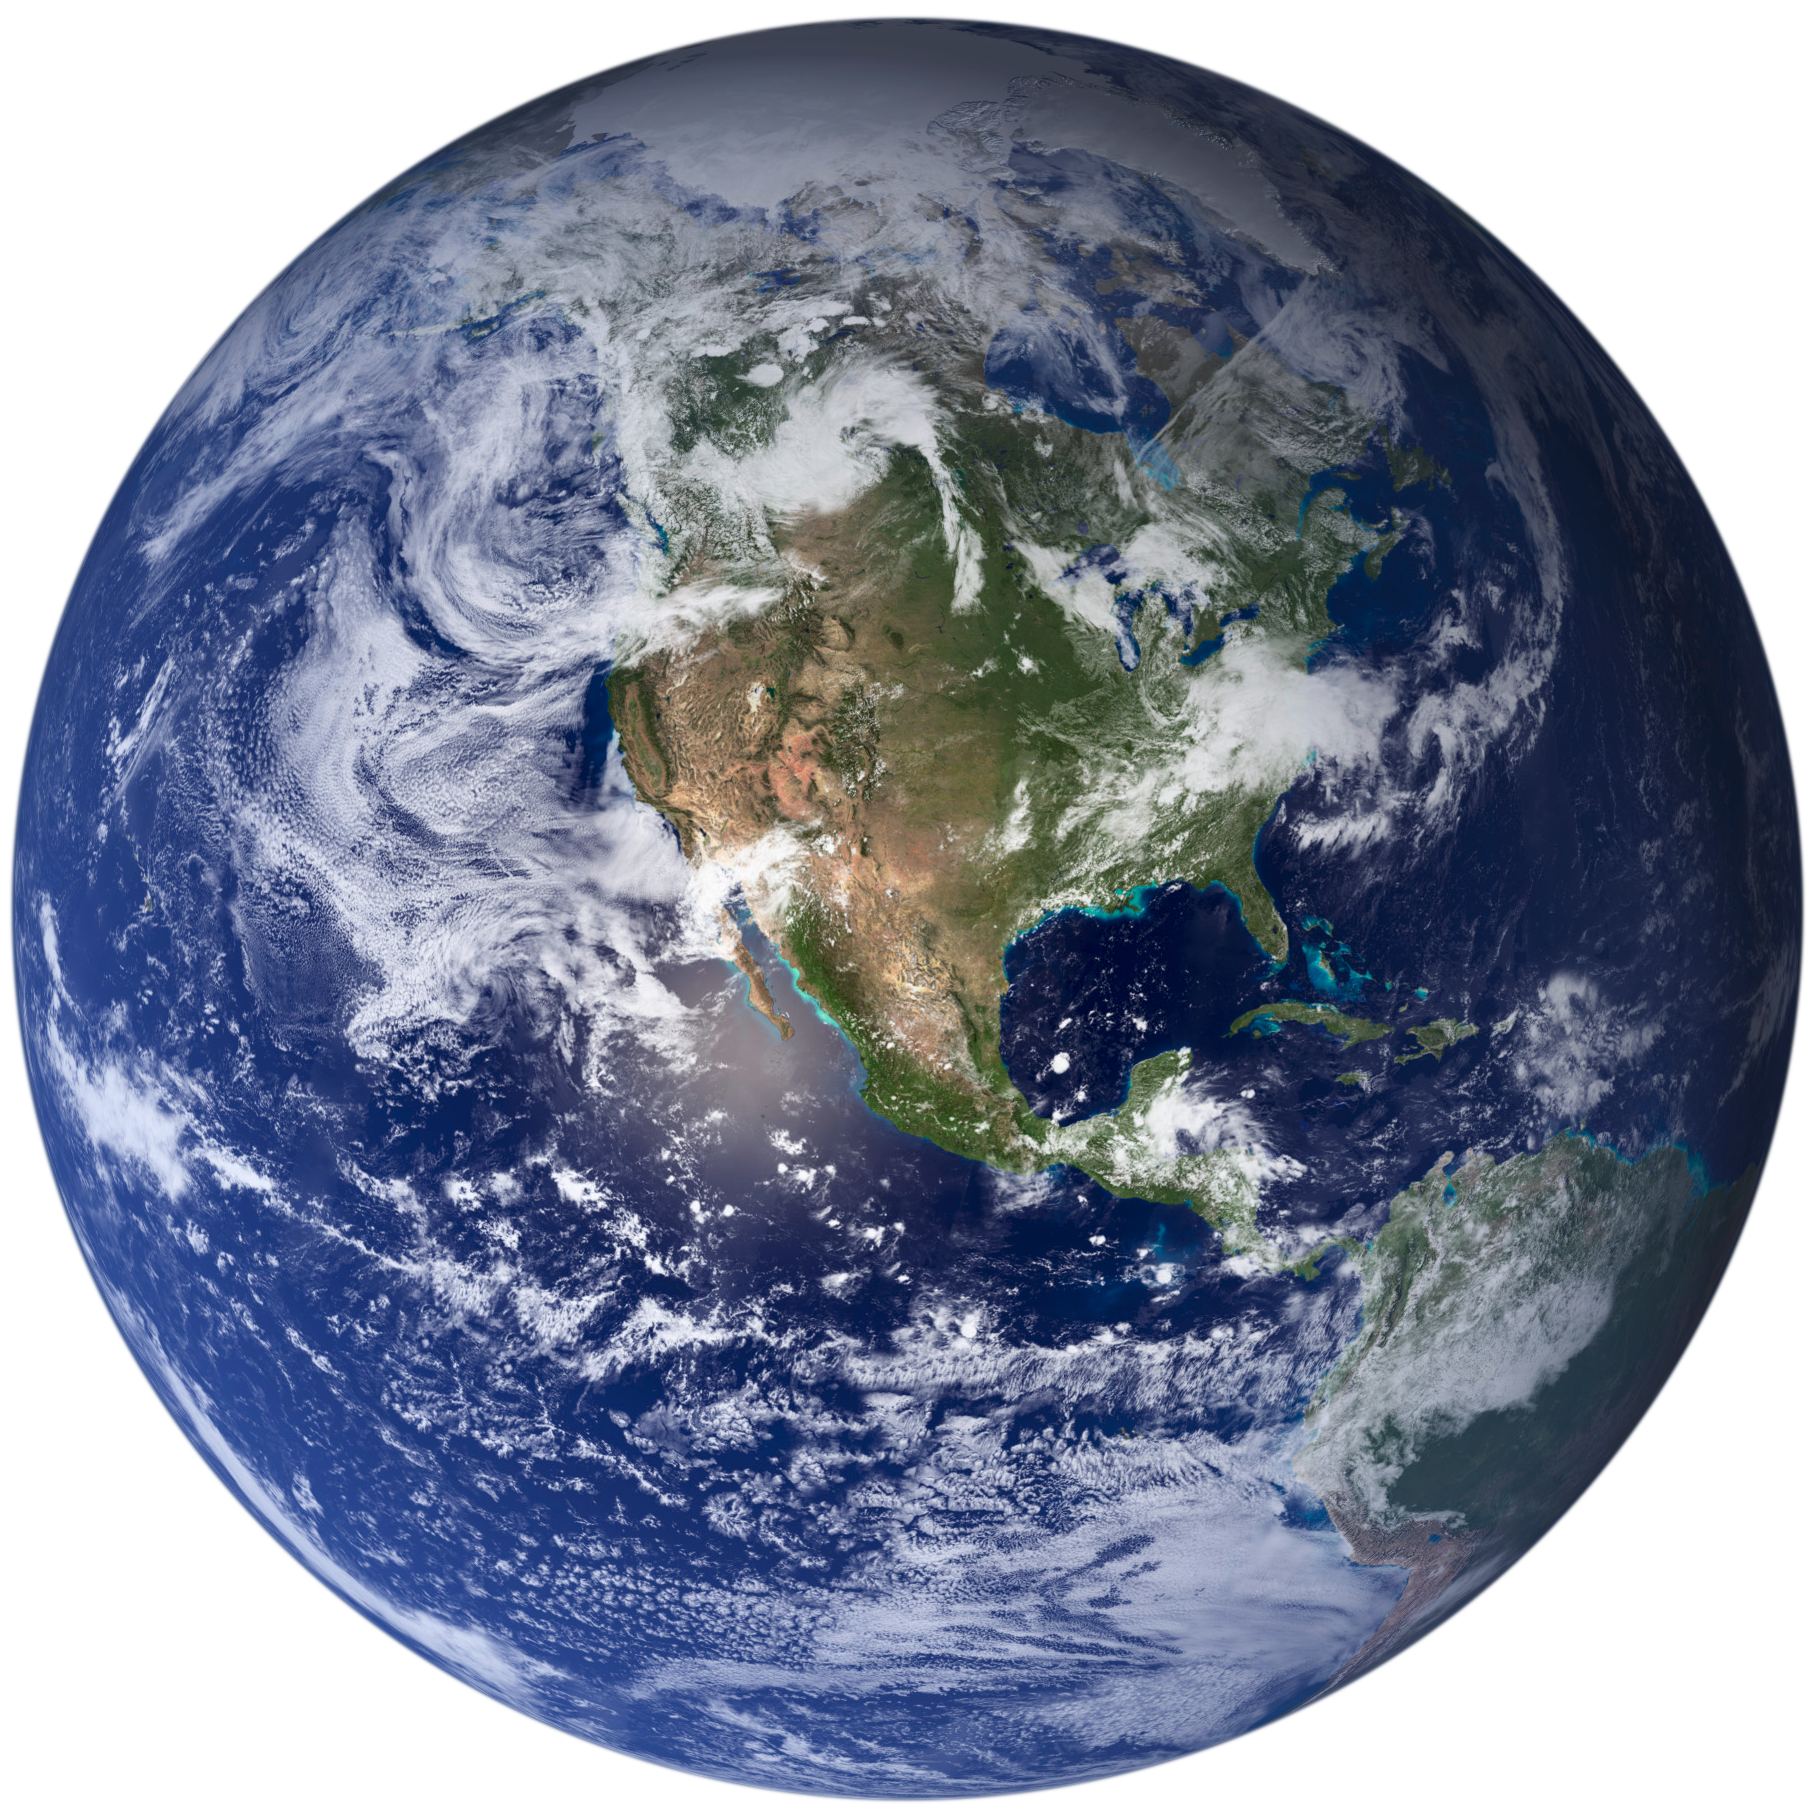
\includegraphics[width=3.0in]{myfigure}
    \caption{Simulation Results}
    \label{simulationfigure}
\end{figure}

\section{Implementation}
At this point, we have successfully developed an algorithm that can be implemented on a computer. However, there are many challenges in actually implementing this algorithm.

\subsection{Design}
Yeah, it was designed.

\subsection{Language Selection}
Yeah, it was selected.

\subsection{Salome}
We chose to use the Salome framework for numerical pre/post-processing. Salome includes a built in geometry system and meshing capabilities.

\subsection{Framework Integration}
Yeah, it was integrated

\subsection{C++ Implementation}
Yeah, it was implemented.

\begin{lstlisting}
#include <stdio.h>
#define N 10
/* Block
 * comment */

int main()
{
    int i;

    // Line comment.
    puts("Hello world!");
    
    for (i = 0; i < N; i++)
    {
        puts("LaTeX is also great for programmers!");
    }

    return 0;
}
\end{lstlisting}

\section{MPI Implementation}
MPI stands for Message Passing Interface and is the \textit{de Facto} standard for implementing parallel algorithms across multiple physical machines.

\section{GPU Implementation}
GPU stands for Graphical Processing Unit and is a collection of SIMD (single instruction multiple data) processors. Each processor operates on its own piece of data but performs the same operation each other processor in its warp is executing.

\section{Conclusion}
Hooray! It works!

\section{Appendix}

\subsection{Laplace's Equation} \label{sec_laplace}
Many physical phenomena can be described by Poisson's Equation given below.

\begin{equation} \label{eq_poisson}
\nabla^2 f = \psi
\end{equation}

Laplace's Equation is a special form of Poisson's Equation and is given by Eq. \ref{eq_laplace}.


\begin{equation} \label{eq_laplace}
\nabla^2 f = 0
\end{equation}

Laplace's equation in cartesian coordinates expands to

\begin{equation} \label{eq_laplace_cartesian}
\nabla^2 f(x, y, z) = \frac{\partial^2 f}{\partial x^2} + \frac{\partial^2 f}{\partial y^2} + \frac{\partial^2 f}{\partial z^2} = 0
\end{equation}

In cylindrical coordinates
\begin{equation} \label{eq_laplace_cylindrical}
\nabla^2 f(r, \phi, z) = \frac{1}{r} \frac{\partial}{\partial r}\left( r \frac{\partial f}{\partial r}\right) + \frac{1}{r^2}\frac{\partial^2 f}{\partial \phi^2} + \frac{\partial^2 f}{\partial z^2}
\end{equation}

In spherical coordinates
\begin{equation} \label{eq_laplace_spherical}
\nabla^2 f(\rho, \theta, \phi) = \frac{1}{\rho^2}\frac{\partial}{\partial \rho} \left( \rho^2 \frac{\partial f}{\partial \rho}\right) + \frac{1}{\rho^2 \sin \theta}\frac{\partial}{\partial \theta}\left( \sin \theta \frac{\partial f}{\partial \theta}\right) + \frac{1}{\rho^2 \sin^2 \theta} \frac{\partial^2 f}{\partial \phi^2}
\end{equation}

Any solution to Laplace's equation is known as a harmonic function. Further, if any two functions are a solution to Laplace's equation, then by the superposition principle, the summation of the two functions is also a solution to Laplace's equation.

Common solutions to Laplace's equation include

\begin{table}
\begin{center}
\label{tbl_laplace_solutions}
\caption{A list of solutions to Laplace's equation in different geometrical systems}
\begin{tabular}{|l|c|}
\hline
Cartesian & Exponential, Circular (a class of trig function), hyperbolic \\ \hline
Cylindrical & Bessel, Exponential, Circular \\ \hline
Spherical & Legendre polynomial, Power, Circular \\ \hline
\end{tabular}
\end{center}
\end{table}

\subsection{Legendre Polynomials} \label{sec_legendre}

Legendre polynomials are solutions to
\begin{equation}
P_n(x) = \frac{1}{2 \pi i} \oint (1-2\xi x + \xi^2)^{-1/2} \xi^{-n-1} d\xi
\end{equation}

\begin{equation}
P_n(x) = \frac{1}{2^n n!}\frac{d^n}{dx^n}(x^2-1)^n
\end{equation}

The first few such solutions are \\
$P_0(x) = 1$ \\
$P_1(x) = x$ \\
$P_2(x) = \frac{1}{2}(3x^2-1)$ \\
$P_3(x) = \frac{1}{2}(5x^3 - 3x)$ \\
$P_4(x) = \frac{1}{8}(35x^4 - 30x^2 + 3)$ \\
$P_5(x) = \frac{1}{8}(63x^5 - 70x^3 + 15x)$ \\
$P_6(x) = \frac{1}{16}(231x^6 - 315x^4 + 105x^2 - 5)$ \\

Associated Legendre polynomials are a generalization of the Legendre polynomial and solve 

\begin{equation}
P_l^m(x) = (-1)^m(1-x^2)^{m/2}\frac{d^m P_l(x)}{dx^m}
\end{equation}

Both Legendre polynomials and Associated Legendre Polynomials can be calculated using the Boost C++ library.

\subsection{Spherical Harmonic Function}

First, we assume that Laplace's equation is of the seperable form $f(\rho, \theta, \phi) = R(\rho)Y(\theta, \phi)$. Equation \ref{eq_laplace_spherical} can then be rewritten as

\begin{equation} \label{eq_spherical1}
\begin{split}
\nabla^2 f(\rho, \theta, \phi) = 
\frac{1}{\rho^2}
\frac{\partial}{\partial \rho} 
\left( \rho^2 \frac{\partial (R(\rho)Y(\theta, \phi))}{\partial \rho}\right) 
+ \\
\frac{1}{\rho^2 \sin \theta}
\frac{\partial}{\partial \theta}
\left( \sin \theta \frac{\partial (R(\rho)Y(\theta, \phi))}{\partial \theta}\right) 
+ 
\frac{1}{\rho^2 \sin^2 \theta} 
\frac{\partial^2 (R(\rho)Y(\theta, \phi))}{\partial \phi^2} = 0
\end{split}
\end{equation}

\noindent
which simplifies to
\begin{equation} \label{eq_spherical2}
\begin{split}
\frac{Y(\theta, \phi)}{\rho^2}
\frac{\partial}{\partial \rho} 
\left( \rho^2 \frac{\partial R(\rho)}{\partial \rho}\right) 
+ 
\frac{R(\rho)}{\rho^2 \sin \theta}
\frac{\partial}{\partial \theta}
\left( \sin \theta \frac{\partial Y(\theta, \phi)}{\partial \theta}\right) 
+ \\
\frac{R(\rho)}{\rho^2 \sin^2 \theta} 
\frac{\partial^2 Y(\theta, \phi)}{\partial \phi^2}
\end{split} = 0
\end{equation}

\noindent
Multiplying Eq. \ref{eq_spherical2} by $\rho^2 / (R(\rho)Y(\theta, \phi))$ yields

\begin{equation}\label{eq_spherical3}
\begin{split}
\frac{1}{R(\rho)}
\frac{\partial}{\partial \rho} 
\left( \rho^2 \frac{\partial R(\rho)}{\partial \rho}\right) 
+ 
\frac{1}{Y(\theta, \phi) \sin \theta}
\frac{\partial}{\partial \theta}
\left( \sin \theta \frac{\partial Y(\theta, \phi)}{\partial \theta}\right) 
+ \\
\frac{1}{Y(\theta, \phi) \sin^2 \theta} 
\frac{\partial^2 Y(\theta, \phi)}{\partial \phi^2} = 0
\end{split}
\end{equation}

Equation \ref{eq_spherical3} can be split into two parts, a function of $\rho$ alone and a component that is a function of $\theta$ and $\phi$ alone. The component that is a function of $\theta$ and $\phi$ can be moved to the other side of the equation. Since two functions of different variables are equal, they must each be equal to some constant, $\lambda$. Therefore, Eq. \ref{eq_spherical3} can be rewritten as two equations:

\begin{equation}\label{eq_spherical_r}
\frac{1}{R(\rho)}
\frac{\partial}{\partial \rho} 
\left( \rho^2 \frac{\partial R(\rho)}{\partial \rho}\right) = \lambda
\end{equation}

\begin{equation}\label{eq_spherical_tp}
\frac{1}{Y(\theta, \phi) \sin \theta}
\frac{\partial}{\partial \theta}
\left( \sin \theta \frac{\partial Y(\theta, \phi)}{\partial \theta}\right) 
+ \\
\frac{1}{Y(\theta, \phi) \sin^2 \theta} 
\frac{\partial^2 Y(\theta, \phi)}{\partial \phi^2} = -\lambda
\end{equation}

$Y(\theta, \phi)$ can be further seperated into $Y(\theta, \phi) = \Theta(\theta)\Phi(\phi)$ which produces

\begin{equation}\label{eq_spherical_y}
\begin{split}
\frac{1}{\Theta(\theta)\Phi(\phi) \sin \theta}
\frac{\partial}{\partial \theta}
\left( \sin \theta \frac{\partial (\Theta(\theta)\Phi(\phi))}{\partial \theta}\right) 
+ \\
\frac{1}{\Theta(\theta)\Phi(\phi) \sin^2 \theta} 
\frac{\partial^2 (\Theta(\theta)\Phi(\phi))}{\partial \phi^2} = -\lambda
\end{split}
\end{equation}

\noindent
which simplifies to

\begin{equation}\label{eq_spherical_y2}
\begin{split}
\frac{1}{\Theta(\theta) \sin \theta}
\frac{\partial}{\partial \theta}
\left( \sin \theta \frac{\partial \Theta(\theta)}{\partial \theta}\right) 
+ 
\frac{1}{\Phi(\phi) \sin^2 \theta} 
\frac{\partial^2 \Phi(\phi)}{\partial \phi^2} = -\lambda
\end{split}
\end{equation}

Multiplying Eq. \ref{eq_spherical_y2} by $\sin^2(\theta)$ and rearranging yields

\begin{equation}\label{eq_spherical_y3}
\begin{split}
\frac{\sin \theta}{\Theta(\theta)}
\frac{\partial}{\partial \theta}
\left( \sin \theta \frac{\partial \Theta(\theta)}{\partial \theta}\right) 
+ \lambda \sin \theta
 = \frac{-1}{\Phi(\phi)} 
\frac{\partial^2 \Phi(\phi)}{\partial \phi^2}
\end{split}
\end{equation}

As before, each side of Eq. \ref{eq_spherical_y3} is a function of a single variable, therefore, both sides are equal to some constant. In this case, we select $m^2$ to be  the constant variable. The produces

\begin{equation}\label{eq_spherical_t}
\begin{split}
\frac{\sin \theta}{\Theta(\theta)}
\frac{\partial}{\partial \theta}
\left( \sin \theta \frac{\partial \Theta(\theta)}{\partial \theta}\right) 
+ \lambda \sin \theta
 = m^2
\end{split}
\end{equation}

\begin{equation}\label{eq_spherical_p}
\begin{split}
\frac{1}{\Phi(\phi)} 
\frac{\partial^2 \Phi(\phi)}{\partial \phi^2} = -m^2
\end{split}
\end{equation}

Combining Eq. \ref{eq_spherical_r}, \ref{eq_spherical_t}, and \ref{eq_spherical_p} Laplace's equation in sperical coordinates can be expressed in a fully seperated form as

\begin{equation}\label{eq_spherical_sep}
\begin{split}
\frac{1}{R(\rho)}
\frac{\partial}{\partial \rho} 
\left( \rho^2 \frac{\partial R(\rho)}{\partial \rho}\right) 
&= \lambda \\
\frac{\sin \theta}{\Theta(\theta)}
\frac{\partial}{\partial \theta}
\left( \sin \theta \frac{\partial \Theta(\theta)}{\partial \theta}\right) 
+ \lambda \sin \theta
&= m^2 \\
\frac{1}{\Phi(\phi)} 
\frac{\partial^2 \Phi(\phi)}{\partial \phi^2}
&= -m^2
\end{split}
\end{equation}

It can be shown through a detailed anlysis that is outside the scope of this paper that $m$ and $\lambda$ must both be integers. $\lambda$ is further constrained in that the relation $\lambda = l(l+1)$ where $l \leq |m|$ and $l \in \mathbb{Z}$. Therefore, Eq. \ref{eq_spherical_sep} can be written as

\begin{equation}\label{eq_spherical_sep2}
\begin{split}
\frac{1}{R(\rho)}
\frac{\partial}{\partial \rho} 
\left( \rho^2 \frac{\partial R(\rho)}{\partial \rho}\right) 
&= l(l+1) \\
\frac{\sin \theta}{\Theta(\theta)}
\frac{\partial}{\partial \theta}
\left( \sin \theta \frac{\partial \Theta(\theta)}{\partial \theta}\right) 
+ l(l+1) \sin \theta
&= m^2 \\
\frac{1}{\Phi(\phi)} 
\frac{\partial^2 \Phi(\phi)}{\partial \phi^2}
&= -m^2 \\
& l, m \in \mathbb{Z} \\
& l \leq |m|
\end{split}
\end{equation}

% TODO
TODO - Discontinuous

It can be shown that the solution is stated

\begin{equation}\label{eq:spherical_harmonic}
Y_l^m(\theta, \varphi) = (-1)^{l}\sqrt{\frac{2l+1}{4 \pi}
\frac{(l-m)!}{(l+m)!}} P_l^m(\cos \theta) e^{im \varphi}
\end{equation}

Using Euler's Equation (Eq. \ref{eq:euler}) to compute the imaginary exponent, the spherical harmonic can be expanded to Eq. \ref{eq:spherical_harmonic_exp}.

\begin{equation}\label{eq:euler}
e^{i \theta} = \cos(\theta) + i \sin(\theta)
\end{equation}

\begin{equation}\label{eq:spherical_harmonic_exp}
Y_l^m(\theta, \varphi) = (-1)^{l}\sqrt{\frac{2l+1}{4 \pi}
\frac{(l-m)!}{(l+m)!}} P_l^m(\cos \theta) \left[ \cos(m \varphi) + i \sin(m \varphi) \right]
\end{equation}

\begin{equation}\label{eq:spherical_harmonic_xs}
\Sigma_s(\Omega \cdot \Omega') \approx \sum_{l=0}^L \sigma_l \sum_{m=-l}^l Y_l^m(\Omega)\bar{Y}_l^m(\Omega')
\end{equation}

where the over-bar denotes the complex conjugate defined by Eq.~\ref{eq:spherical_harmonic_conj}.

\begin{equation}\label{eq:spherical_harmonic_conj}
\bar{Y}_l^m(\theta, \varphi) = (-1)^{l}\sqrt{\frac{2l+1}{4 \pi}
\frac{(l-m)!}{(l+m)!}} P_l^m(\cos \theta) \left[ \cos(m \varphi) - i \sin(m \varphi) \right]
\end{equation}

Expanding the inner summation of \ref{eq:spherical_harmonic_xs} with Eq.~\ref{eq:spherical_harmonic_exp} and \ref{eq:spherical_harmonic_conj} yields:

\begin{equation}\label{eq:spherical_harmonic_xs_inner}
\begin{split}
Y_l^m(\theta, \varphi)\bar{Y}_l^m(\theta', \varphi') & = 
(-1)^{2l}\frac{2l+1}{4 \pi}
\frac{(l-m)!}{(l+m)!} P_l^m(\cos \theta) P_l^m(\cos \theta') \times \\
&\left[ \cos(m \varphi) + i \sin(m \varphi) \right] \left[ \cos(m \varphi') - i \sin(m \varphi') \right] \\
& = \frac{2l+1}{4 \pi}
\frac{(l-m)!}{(l+m)!} P_l^m(\cos \theta) P_l^m(\cos \theta') \times \\
& \left[ \cos(m \varphi) \cos(m \varphi') + i \sin(m \varphi)\cos(m \varphi') - i \sin(m \varphi') \cos(m \varphi) - i^2\sin(m \varphi) \sin(m \varphi') \right]
\end{split}
\end{equation}

The real part of the

whose real part can be expanded to

\begin{equation}
Y_l^0 = \sqrt{\frac{2l+1}{4 \pi}}P_l^0(1)
\end{equation}

\begin{equation}
Y_l^{m, even} = (-1)^m\sqrt{\frac{2l+1}{2 \pi} \frac{(l-m)!}{(l+m)!}}P_l^m(\cos(m \phi))
\end{equation}

\begin{equation}
Y_l^{m,odd} = (-1)^m \sqrt{\frac{2l+1}{2 \pi} \frac{(l-m)!}{(l+m)!}}P_l^m(\sin(m \phi))
\end{equation}

Some useful recurrence relations used to calculate the Associated Legendre Polynomials are:

\begin{equation}
P_l^l(x) = (-1)^l(2l-1)!!(1-x^2)^(l/2)
\end{equation}

\begin{equation}
P_{l+1}^l(x) = x(2l+1)P_l^l(x)
\end{equation}

\begin{equation}
P_l^l(x) = (-1)^l(2l-1)!!(1-x^2)^(l/2)
\end{equation}

where $x!!$ is the double factorial function defined by:

\begin{equation}
x!! = \prod_{k=0}^{\lceil x/2 \rceil - 1} x-2k
\end{equation}

For example, $5!! = 5 \times 3 \times 1 = 15$.

\subsection{Klein-Nishina Formula}

The Klein-Nishina formula gives the differential scattering cross section of photon incident on a single free electron.

\begin{equation}\label{klein_nishina}
\frac{\partial \sigma}{\partial \Omega} = \frac{1}{2}\alpha^2 r_c^2 P(E_\gamma, \theta)^2
\left( P(E_\gamma, \theta) + P(E_\gamma, \theta)^{-1} - 1 + \cos^2(\theta) \right)
\end{equation}

\begin{equation}\label{klein_nishina2}
P(E_\gamma, \theta) = \frac{1}{1 + (\frac{E_\gamma}{m_e c^2})(1-\cos(\theta))}
\end{equation}


\noindent
where $\alpha$ is the fine structure constant ($\alpha \approx 7.2971E-3$), $r_c$ is the reduced Compton wavelength ($r_c = \hbar$)

\subsection{Numeric Integration}

\begin{equation}
\tilde{H}
\end{equation}

\end{document}